Here's quite a beautiful probability problem with a decent story behind it.

\begin{blackbox}
    \begin{problem}
        Let \( x_1, x_2, \ldots, x_n \) be random variables chosen uniformly
        from the interval \( \left[0, 1\right] \). What is the probability that
        \[
            x_1 + x_2 + \cdots + x_n \geqslant 1
        ?\]
    \end{problem}
\end{blackbox}

Originally this was supposed to be Entry 007 in the journal, but for the
longest time I had been working on the problem and hadn't gotten a solution. It
was only in the summer after talking with some friends and thinking about it on
and off for around a week or two that I made progress and realized a bunch of
different things. As such, I've felt it only fair to move it to the end and
change the journal entry date to match when I'm actually writing this now.

One of the things that makes solving this problem potentially fun is, if you're
more familiar with contest math probability problems, they usually turn out to
be more discrete in nature. What makes this problem a breath of fresh air in a
way is that it's continuous, and one can't really reduce it to a combinatorics
problem. \MarginComment{Ah yes my favorite style of proof: proof by exhaustion
on the real numbers.} This certainly encourages a different way to go about
problem solving. Case work is instead transformed into different methods of
attacking the problem.

In total, this problem is a really great example of how the journey matters far
more than the destination. When I was looking for different ways to approach
the problem, I knew full well the correct answer already. While I certainly
think the final result is interesting in itself, I had the most fun simply
talking with friends about the problem, researching different solution
strategies, visualizing 4D, falling down a rabbit hole involving simplices,
learning about probability distributions, and so much other stuff.

I hope you enjoy this problem even a little as much as I did!

% Ok ok hopefully I can take the time to make a bunch of pictures with tikz.

\subsection{Intuiting the Problem}

% Talk about the intuition in terms of the sliders from 0 to 1 that Kelly gave.
% In addition, a good geometric image for what's happening might be putting
% these sliders orthogonal to each other to create our n-dimensional cube.

% Write about the sorts of conditions a solution would have (as we go to
% infinity, the probability should go to 1). Talk about how the complement will
% also be important later on.

% Draw pictures of sliders (and their sliders in some place and the sum,
% representing one realization of the random result) and then put them on a
% cube maybe.

Before I jump into any solutions or a bunch of math, let's first take a moment
to really digest what the problem is asking for. Imagine we have \( n \)
sliders going from \( 0 \) to \( 1 \), \MarginComment{\begin{center}
    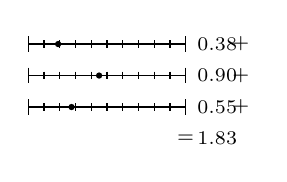
\begin{tikzpicture}
        \foreach \y in {0, -0.4, -0.8} {
            \draw (0, \y) -- (2, \y);

            \draw (0, \y + 0.1) -- (0, \y - 0.1);
            \draw (2, \y + 0.1) -- (2, \y - 0.1);
            \foreach \x in {0.2, 0.4, ..., 1.8} {
                \draw (\x, \y + 0.05) -- (\x, \y - 0.05);
            }
        }

        \fill (0.38, 0) circle (0.04);
        \fill (0.9, -0.4) circle (0.04);
        \fill (0.55, -0.8) circle (0.04);

        \node at (2.4, 0) {\scriptsize \( 0.38 \)};
        \node at (2.4, -0.4) {\scriptsize \( 0.90 \)};
        \node at (2.4, -0.8) {\scriptsize \( 0.55 \)};

        \node at (2.7, 0) {\scriptsize \( + \)};
        \node at (2.7, -0.4) {\scriptsize \( + \)};
        \node at (2.7, -0.8) {\scriptsize \( + \)};

        \node at (2.4, -1.2) {\scriptsize \( 1.83 \)};
        \node at (2.0, -1.2) {\scriptsize \( = \)};
    \end{tikzpicture}
\end{center}
\captionof{figure}{One realization of the state of the sliders and their sum for \( n = 3 \). We see that this state is included in the set of solutions for which the sum is greater than \( 1 \).}
} which we can freely move around and
adjust to our choosing. We can scramble these sliders however we want, and
after we're done, we take the sum of the sliders and check whether it's less
than \( 1 \) or greater than \( 1 \). We want to know the probability that
after scrambling these sliders in any sort of way, we get a sum greater than \(
1 \).

One thing to note is that frequently throughout the different solution methods,
we consider the complement of the probability as it is far easier to work with
for some geometric solutions. When talking about the complement, we are
referring to the probability that the sum is less than \( 1 \). (In fact, I actually considered changing around the problem to directly look at the complement, but in ordered to better encapsulate my progression throughout the entire problem and such, I deemed it better to simply leave the original problem statement how I found it. Perhaps this might change in the future if I ever find myself mulling over it too much.)

Another thing to note is that, rather intuitively, the probability should
increase as we increase \( n \), as there is a greater and greater chance of
the sum being greater than \( 1 \). This means that our desired closed form for
the probability should approach \( 1 \) as \( n \to \infty \). Working in
tandem, this means our complement probability (the probability that the sum is
less than \( 1 \)), shall approach \( 0 \).

% Talk about how throughout we may go between looking at a slider view as wella
% s a more geometric view (explore more into R^n and all that and how putting
% the sliders orthogonally represents this).

\subsection{Calculus Methods}

% Talk about *the integral* some of the smaller techniques I tried to use to
% solve it (like the min, max, filling the cube stuff) as well as some worked
% out examples of smaller dimensions to show that it doesn't seem to be viable

% At the end should be a short section on how I would like to show Max's proof
% of it, but I don't fully understand the proof right now, so I can't do it
% justice.

\subsection{Geometric Methods}

% Explain the slight difference between calculus and geometric methods
% (although the line certainly is blurry). Talk about the different attempts to
% "fill" a shape with simplices. Oh boy talk about simplices. Finally, talk
% about how I eventually ended up at a solution that was right in front of me
% the entire time, although perhaps not the most satisfactory as it makes some
% assumptions that might be a little hmmmm.

\subsubsection{A Not So Brief Interlude On Simplices}

\begin{figure}
    \begin{minipage}{0.24\textwidth}
    \centering
    \begin{tikzpicture}
        \node[label={[anchor=west]:\tiny \( \left( 1, 0, 0 \right) \)}] (xbasis) at (1, 0, 0) {};
        \node[label={[anchor=west]:\tiny \( \left( 0, 1, 0 \right) \)}] (ybasis) at (0, 1, 0) {};
        \node[label={[anchor=north west]:\tiny \( \left( 0, 0, 1 \right) \)}] (zbasis) at (0, 0, 1) {};

        \fill[fadegray, opacity=0.5] (xbasis.center) -- (ybasis.center) -- (zbasis.center) -- cycle;

        \fill (xbasis) circle (0.05cm);
        \fill (ybasis) circle (0.05cm);
        \fill (zbasis) circle (0.05cm);

        \draw (xbasis.center) -- (ybasis.center);
        \draw (xbasis.center) -- (zbasis.center);
        \draw (ybasis.center) -- (zbasis.center);


        \draw[->] (0, 0, 0) -- (1.5, 0, 0);
        \draw[->] (0, 0, 0) -- (0, 1.5, 0);
        \draw[->] (0, 0, 0) -- (0, 0, 1.5);
    \end{tikzpicture}
    \end{minipage}
    \begin{minipage}{0.24\textwidth}
    \centering
    \tdplotsetmaincoords{70}{-90} % 70 -45
    \begin{tikzpicture}[tdplot_main_coords]
        \node[label={[anchor=west]:\tiny \( \left( 1, 0, 0 \right) \)}] (xbasis) at (1, 0, 0) {};
        \node[label={[anchor=south]:\tiny \( \left( 0, 1, 0 \right) \)}] (ybasis) at (0, 1, 0) {};
        \node[label={[anchor=west]:\tiny \( \left( 0, 0, 1 \right) \)}] (zbasis) at (0, 0, 1) {};

        \fill[fadegray, opacity=0.5] (xbasis.center) -- (ybasis.center) -- (zbasis.center) -- cycle;

        \fill (xbasis) circle (0.05cm);
        \fill (ybasis) circle (0.05cm);
        \fill (zbasis) circle (0.05cm);

        \draw (xbasis.center) -- (ybasis.center);
        \draw (xbasis.center) -- (zbasis.center);
        \draw (ybasis.center) -- (zbasis.center);


        \draw[->] (0, 0, 0) -- (1.5, 0, 0);
        \draw[->] (0, 0, 0) -- (0, 1.5, 0);
        \draw[->] (0, 0, 0) -- (0, 0, 1.5);
    \end{tikzpicture}
    \end{minipage}
    \begin{minipage}{0.24\textwidth}
    \centering
    \tdplotsetmaincoords{70}{-180} % 70 -45
    \begin{tikzpicture}[tdplot_main_coords]
        \node[label={[anchor=south]:\tiny \( \left( 1, 0, 0 \right) \)}] (xbasis) at (1, 0, 0) {};
        \node[label={[anchor=west]:\tiny \( \left( 0, 1, 0 \right) \)}] (ybasis) at (0, 1, 0) {};
        \node[label={[anchor=west]:\tiny \( \left( 0, 0, 1 \right) \)}] (zbasis) at (0, 0, 1) {};

        \fill[fadegray, opacity=0.5] (xbasis.center) -- (ybasis.center) -- (zbasis.center) -- cycle;

        \fill (xbasis) circle (0.05cm);
        \fill (ybasis) circle (0.05cm);
        \fill (zbasis) circle (0.05cm);

        \draw (xbasis.center) -- (ybasis.center);
        \draw (xbasis.center) -- (zbasis.center);
        \draw (ybasis.center) -- (zbasis.center);


        \draw[->] (0, 0, 0) -- (1.5, 0, 0);
        \draw[->] (0, 0, 0) -- (0, 1.5, 0);
        \draw[->] (0, 0, 0) -- (0, 0, 1.5);
    \end{tikzpicture}
    \end{minipage}
    \begin{minipage}{0.24\textwidth}
    \centering
    \tdplotsetmaincoords{70}{-45} % 70 -45
    \begin{tikzpicture}[tdplot_main_coords]
        \node[label={[anchor=south]:\tiny \( \left( 1, 0, 0 \right) \)}] (xbasis) at (1, 0, 0) {};
        \node[label={[anchor=south]:\tiny \( \left( 0, 1, 0 \right) \)}] (ybasis) at (0, 1, 0) {};
        \node[label={[anchor=east]:\tiny \( \left( 0, 0, 1 \right) \)}] (zbasis) at (0, 0, 1) {};

        \fill[fadegray, opacity=0.5] (xbasis.center) -- (ybasis.center) -- (zbasis.center) -- cycle;

        \fill (xbasis) circle (0.05cm);
        \fill (ybasis) circle (0.05cm);
        \fill (zbasis) circle (0.05cm);

        \draw (xbasis.center) -- (ybasis.center);
        \draw (xbasis.center) -- (zbasis.center);
        \draw (ybasis.center) -- (zbasis.center);


        \draw[->] (0, 0, 0) -- (1.5, 0, 0);
        \draw[->] (0, 0, 0) -- (0, 1.5, 0);
        \draw[->] (0, 0, 0) -- (0, 0, 1.5);
    \end{tikzpicture}
    \end{minipage}
    \caption{Different views of a \( 3 \)-simplex.}
\end{figure}


% Talk about simplices from the definition and the geometric point of view and
% how they play a major role in this problem. Focus on standard simplices of
% course. 
% One has to be careful of how they talk about simplices because a
% (k+1)-simplex is the boundary of (k + 1) vertices, which makes it k
% dimensional (topologists lmao). What we really want to talk about is the
% volume of the simplex.

\subsection{Algebraic Methods}

% Talk about potential linear algebra solutions (the one given on wikipedia
% although the arguments look very similar except the MSE answer has a bit more
% explanation) as well as the answer given by (I found this right now lmao)
% https://math.stackexchange.com/questions/1718021/intuition-for-volume-of-a-simplex-being-frac-1n
% ^ Essentially, using linear algebra, we can use a linear transformation with
% determinant 1 to transform the probability problem of real numbers adding up
% to 1 to a probability problem of real numbers being sorted.

\subsection{Probabilistic Methods}

% What I need to write here pretty much lives rent free in my brain, so there
% isn't too much need to explain it, but perhaps I shall put down some lines
% here that I want to remember.
% Make sure to write about the extra merits of this solution, the major one
% being it is a bit more general and far more extensible.

This is where the real spicy stuff happens, and where I believe this problem
truly shines. It's in fact this solution that I came up over the course of a
couple days which really inspired me to get more interested in probability
\MarginComment{Expect more probability journal entries soon? ;)} (especially
probability distributions) as well as mathematical statistics.

\begin{figure}
    \centering
    \begin{tikzpicture}[
        flowbox/.style={rectangle, text centered, minimum width=1cm, minimum height=0.5cm, draw=black, font={\tiny}},
        flowarrow/.style={->}
    ]
        \node[flowbox] (start) {Start};
        \node[flowbox, right of=start, xshift=1cm] (udists) {Uniform Distributions};
        \node[flowbox, right of=udists, xshift=2cm] (tdist) {Total Distribution};
        \node[flowbox, right of=tdist, xshift=1cm] (answer) {Answer};

        \node (middle) at ($(udists.east)!0.5!(tdist.west)$) {};

        \node[flowbox, below of=middle, yshift=-0.1cm] (lap) {Laplace World};

        \draw[flowarrow] (start) -- (udists);
        \draw[flowarrow, decorate, decoration={zigzag, segment length=0.19cm, amplitude=0.05cm}] (udists) -- node[anchor=south, scale=0.8] {\tiny Convolutions} (tdist);
        \draw[flowarrow] (tdist) -- (answer);

        \draw[flowarrow] (udists) -- node[anchor=east] {\tiny \( \LaplaceL \)} (lap.west);
        \draw[flowarrow] (lap.east) -- node[anchor=west] {\tiny \( \InvLaplaceL \)} (tdist);
    \end{tikzpicture}
    \caption{The solution path for solving the problem using probabilistic methods. Convolutions are too hard to work with even for small \( n \), but we can sidestep them with Laplace transforms.}
\end{figure}



\subsection{Some Afterthoughts}

% Talk about how we can transform to product using AM-GM inequality.
% Except this doesn't actually preserve the probability so should it even be mentioned here?
% Perhaps I can treat it as a different problem with a similar style and then
% talk about more generalizations of the original problem.
